%% -*-LaTeX-*-
%%
%% This manuscript has been written using the IEEEtran macros
%% To be submitted to: Open Source Modelling and Simulation of Energy Systems
%% (OSMSES 2022)
%%
%% (c) 2021 Grupo AIA, RTE  
%%
%% 
%%

\documentclass[conference]{IEEEtran}
\usepackage[utf8]{inputenc}
\usepackage{hyperref}
\usepackage{graphicx}
\usepackage{booktabs}
\usepackage{cite}
\usepackage[cbgreek]{textgreek} % Only for Dynawo "omega" font
\usepackage{xcolor}
\usepackage[mode=text]{siunitx}


%%%%%%%%%%%%%%%%%%%%%%%%%%%%%%%%%%%%%%%%%%%%%%%%%%%%%%%%%%%%%%%%%%%%%%%%%%%%%%%
%% Our short-hand macros
\newcommand{\Dynawo}{Dyna\textomega o} % unfortunately, it doesn't show in bold

%% Our colors for backgrounds and code listings
\definecolor{light-gray}{gray}{0.9}
\definecolor{dark-gray}{gray}{0.4}
\definecolor{light-blue}{RGB}{64,64,255}
\definecolor{dark-blue}{RGB}{16,16,64}

%% Our short-hand macros for code snippets:
\newcommand{\code}[1]{\texttt{#1}}

%% More sensible colors for hyperref links
\hypersetup{
  colorlinks = true, % color links instead of ugly boxes
  urlcolor   = blue, % color of external hyperlinks
  linkcolor  = dark-blue, % color of internal links
  citecolor  = red   % color of citations
}




%%%%%%%%%%%%%%%%%%%%%%%%%%%%%%%%%%%%%%%%%%%%%%%%%%%%%%%%%%%%%%%%%%%%%%%%%%%%%%%%
\begin{document}

%% Used by IEEEtran.bst to control some aspects of the bibliography style:
\bstctlcite{BSTcontrol}

% Remember: no symbols, special chars, footnotes, or math in Title or Abstract
\title{An Open Source Tool to Compare Simulators on Large-Scale Cases
  --- Application to Dynawo}

\author{
  \IEEEauthorblockN{
    Jose Luis Marin\IEEEauthorrefmark{1},
    Vicenç Gaitan\IEEEauthorrefmark{1},
    Guiu Oms\IEEEauthorrefmark{1},
    Marco Chiaramello\IEEEauthorrefmark{2},
    Quentin Cossart\IEEEauthorrefmark{2}
    and Adrien Guironnet\IEEEauthorrefmark{2}}
  \IEEEauthorblockA{
    \IEEEauthorrefmark{1}Aplicaciones en Informática Avanzada SL, Avda.\ de la
    Torre Blanca 57, 08172 Sant Cugat del Vallès, Spain\\
    \{marinjl, gaitanv, omsg\}@aia.es}
  \IEEEauthorblockA{
    \IEEEauthorrefmark{2}R\&D department, RTE Réseau de Transport d’Electricité,
    Paris, France\\
    \{marco.chiaramello, quentin.cossart, adrien.guironnet\}@rte-france.com}
}

\maketitle

% Remember: no symbols, special chars, footnotes, or math in Title or Abstract
\begin{abstract}
  Dynawo is an open source hybrid Modelica/C++ suite of simulation tools for
  power systems, geared towards the time-domain simulation of large transmission
  networks at different time scales, from the steady-state calculation to
  transient stability analysis. In this paper a set of open source tools is
  presented, designed for: (a) validation of Dynawo based on black-box testing
  against existing established simulators, or against previous validated
  versions of Dynawo; (b) exploration and analysis of the effects of modelling
  changes and model parameters on the network response, by means of A/B
  testing. In both cases the approach is based on the automatic generation of an
  extensive set of cases derived from a given base case, typically by means of
  N-1 contingencies. Most importantly from the point of view of power systems
  research, a concrete set of metrics is presented to deal with the practical
  problems of comparing different simulations of large, real-world systems. The
  tools, based on Python and Jupyter notebooks, are designed with flexibility in
  mind, in order to adapt the code to future testing scenarios and to extend the
  metrics used for comparing results.
\end{abstract}

\begin{IEEEkeywords}
  equation based modelling, time-domain simulation, power flow, blackbox validation
\end{IEEEkeywords}




%%%%%%%%%%%%%%%%%%%%%%%%%%%%%%%%%%%%%%%%%%%%%%%%%%%%%%%%%%%%%%%%%%%%%%%%%%%%%%%%
\section{Introduction and context}

\Dynawo{}~\cite{Guironnet18} is a suite of tools for the time-domain simulation,
at different time resolution levels, of modern power networks.  It has been
mainly developed by RTE, and then released as open source.\footnote{Available
  at: \url{https://dynawo.github.io}} Its design is based on two major guiding
principles: the use of a high-level modelling language
(Modelica~\cite{Modelica}) and a strict separation between the modelling and the
solving mechanisms.  Its implementation brings to the table a novel hybrid
approach that combines the power of declarative, computationally acausal
modelling (also referred to as equation-based modelling) with certain
high-performance C/C++ modifications that take advantage of the specific
optimization opportunities available in large power networks (such as, for
instance, the extensive work on high-performance Differential Algebraic
Equations (DAE) solvers for these highly sparse systems).  \Dynawo{} aims to be
a next-generation open source suite of simulation tools that overcomes the
limitations of legacy closed-source programs, while being performant enough to
be used in production settings at large transmission operators. The key goals
are transparency and modelling flexibility, which results in interoperability
and robustness. It is hoped that this will enable an effective collaboration and
cooperation in the power system community, something that has proven notoriously
difficult using legacy commercial tools.  For a recent update on \Dynawo{}
developments, see the presentation \cite{Guironnet21} or consult the official
website.



\subsection{Objectives of the developed comparison tools}

Validation of time-domain simulators is difficult, and it starts at the level of
individual device models. Since these devices are increasingly more complex
(with new power electronics) and sometimes governed by algorithmic controls, one
needs \emph{whole-system functional testing} in order to assess the behaviour on
complete network cases. As in any hierarchical system-of-systems, it is not
always evident how the lower-level details (device model choices, parameters,
etc.)  affect the behaviour of the whole network. This sort of testing is
necessarily black-box in style, as there is no systematic way to link the
knowledge of the lower-level modelling to the behaviour of the higher-level,
other than running simulations.  Therefore black box simulations are not only
useful for validating the software against previous legacy simulators, or
against new versions of the software, but also for exploring and assessing the
effects of different model choices, model parameters, solver parameters, etc.,
on the behaviour of the whole network, \emph{in a systematic way}.

The tools presented here aim to fulfill this double role. They leverage modern
components from the Python ecosystem (Pandas and Jupyter notebooks for instance)
to automatically generate extensive sets of test cases derived from a given base
case, and efficiently manage large amounts of outputs. Initially developed for
the validation of \Dynawo{} at the functional level, they are now also used for
the exploration of extensive sets of test cases, which could consist of full N-1
contingency sweeps or user-provided sets (see~\cite{Bogodorova20} as an example
of how to generate statistically representative samples of N-k contingencies).

But besides efficient data-handling, the two key ingredients are the design of
an adequate set of \emph{metrics} for comparing the results from two simulators,
and the selection of \emph{effective visualization} techniques for the analysis.
These are non-trivial problems that required experimenting with different
choices. A collateral benefit is that these analysis tools can easily be
repurposed for screening contingencies.

This paper describes the tools and reports on our early experience using them on
large network cases (actual cases from RTE's operational environment). The two
\Dynawo{} simulators for which they have been constructed, \emph{DynaWaltz}
(long-term stability studies) and \emph{DynaFlow} (power flow via time-domain
simulation), are first presented.



\subsection{About DynaWaltz and DynaFlow}

\Dynawo{} is flexible enough to accommodate several time scales: from sub-second
near-EMT (Electro-Magnetic Transients)~\cite{Masoon21}, to long-term stability,
to steady-state calculation~\cite{Cossart21} studies. DynaWaltz is \Dynawo{}
when used for long-term stability studies, where the time scales are measured in
minutes and the typical time steps can be of the order of a few seconds. Used in
this mode, \Dynawo{} simulates the grid in the so-called quasi steady state, by
adopting the models that have most impact on the system slow dynamics:
tap-changers, loads, static var compensators, etc.; as well as secondary voltage
regulation and special protection schemes. It is mostly used to study voltage
collapses. Other possible uses in the future may include cascading failure
analysis~\cite{Bialek16}.

The validation tools described here have been developed to assess and validate
DynaWaltz quantitatively and in a systematic manner, using RTE's national grid
models and cases in the context of long-term stability studies. Initially, the
approach was based on comparing against another well-established
simulator, \emph{Astre}, which is the current production tool. More
specifically, the validation focused on the behaviour of the coordinated
Secondary Voltage Control (SVC) systems. Shortly after, the tools have been
extended to accommodate the comparison between different \Dynawo{} versions, or
between variations of models, model parameters, and solver parameters. As
DynaWaltz is scheduled to be deployed in production at RTE starting in late
2021, these tools become an important enabler of ongoing evolution and change.

DynaFlow~\cite{Cossart21}, on the other hand, is a novel approach to the
calculation of steady states that leverages \Dynawo's flexibility for modelling
the dynamics at different time scales. It overcomes an inherent problem that all
static power flows have dealing with controls: discrete event actions,
dead-bands, and regulation limits (control type-switching) conspire to produce
several possible steady-state solutions, many of them operationally valid.
Static power flows arrive at a single solution by means of several ``outer
loops'' in which heuristics (accumulated over years of practice) drive the
choice of control changes. However, these heuristics are not bullet-proof (for
instance, one may encounter ``hunting'' oscillations, even with standard tap
changers); and more importantly, they do not take into account the time
constants and actual dynamics of each control. Therefore, even the most
principled approaches from the static camp, such as those based on
optimization\cite{Ju20}, complementarity constraints~\cite{Murray15}, or
HELM~\cite{Trias18} cannot guarantee arriving at the correct solution, since
they are blind to the dynamics of competing controls.

In the current scenario, where more complex power electronic devices and
algorithm-based controls are being introduced each year, this problem is getting
worse. DynaFlow overcomes these problems by simulating the network in the time
domain and using the actual time constants that govern the actions of relevant
controls. It also contemplates protection schemes, including modern Special
Protection Schemes (SPS), thus opening the door to the realistic simulation of
cascading effects in contingency studies.

Following the work done for DynaWaltz, a similar set of tools has been built for
DynaFlow.  Again, the approach to validation is based on comparison against a
well-established power flow, \emph{Hades}, currently in production at RTE. The
tool is also prepared for comparing different DynaFlow versions, and more
generally, for assessing the effects of varying the case models, model
parameters, and solver parameters.




%%%%%%%%%%%%%%%%%%%%%%%%%%%%%%%%%%%%%%%%%%%%%%%%%%%%%%%%%%%%%%%%%%%%%%%%%%%%%%%%
\section{Structure and workflow}

The validation approach is based on comparing results against a well-known
reference simulator, in this case Astre for the validation of DynaWaltz and
Hades for the validation of DynaFlow. The cases used for comparison are
essentially all possible single-element disconnections (shunts, lines,
etc.). Therefore, the tools are currently oriented towards the generation of
contingency cases derived from a given base case. However, the design is quite
modular; it is easy to modify the corresponding scripts so that the test set
would be something other than contingencies; such as, for instance, variations
of a given set of model parameters, or the solver time-step, etc.

The typical workflow is:
\begin{enumerate}
  \item Obtain a study case containing the two set of files that represent the
        same case (i.e.~the DynaWaltz and Astre files, or the DynaFlow and Hades
        files); these will be the base for A/B comparison;
  \item Prepare the base case: standardize the folder and file structure (see
        below), the XML formatting, and possibly some case-specific input (such as,
        which curves to extract, for instance);
  \item Create the contingency cases derived from the base case: for each type
        of device whose disconnection is supported (shunts, loads, generators,
        lines, transformers), create the specified number of single-contingency
        cases.
  \item Run Astre and DynaWaltz (or Hades and DynaFlow) on the contingency
        cases, collect results and logs into organized (and compressed)
        storage;
  \item Extract result data in a format common to Astre and DynaWaltz (or Hades
        and DynaFlow);
  \item Compute \emph{metrics} on the obtained results (this requires having
        selected adequate variables and careful design of the metrics to apply);
  \item Use the provided Jupyter notebook to browse and analyze the results.
        Obtain lists of contingency cases that can be ranked according to various
        compound scores built on those metrics;
  \item Further analysis is possible using these ranked tables that
        the notebook exports to CSV files (e.g. using Excel).
\end{enumerate}

Steps 1 and 2 are semi-manual, aided by a few helper scripts.  One should
firstly make sure that the A/B files do correspond to the same case. This is
relatively easy when both cases are \Dynawo, but challenging when the simulators
are different.  One needs not only the underlying network model to be the same,
but additionally the identifiers of at least the most basic elements (buses,
loads, generators, etc.) to be the same, or provide a dictionary to match them.
By experience, having a single-source asset database feeding the creation of
both files is not enough to find a \SI{100}{\%} match for all elements---there
would always be a small number of non-matching devices, such as, for instance,
merged loads, or bus-branch vs.\ node-breaker representations. Therefore the
tools take this into account, only disconnecting elements and comparing
variables that can unequivocally be matched.

Beginning with Step 3, the rest of this workflow has been automated through a
series of Python programs and Bash shell scripts. In this paper, this system is
referred to as the \emph{process pipeline} for validation. This is depicted
schematically in Fig.~\ref{fig:pipeline1}. Each script in this pipeline can also
be run individually, either for debugging purposes or just because one wants to
run the pipeline manually step by step.

\begin{figure}
  \centering
  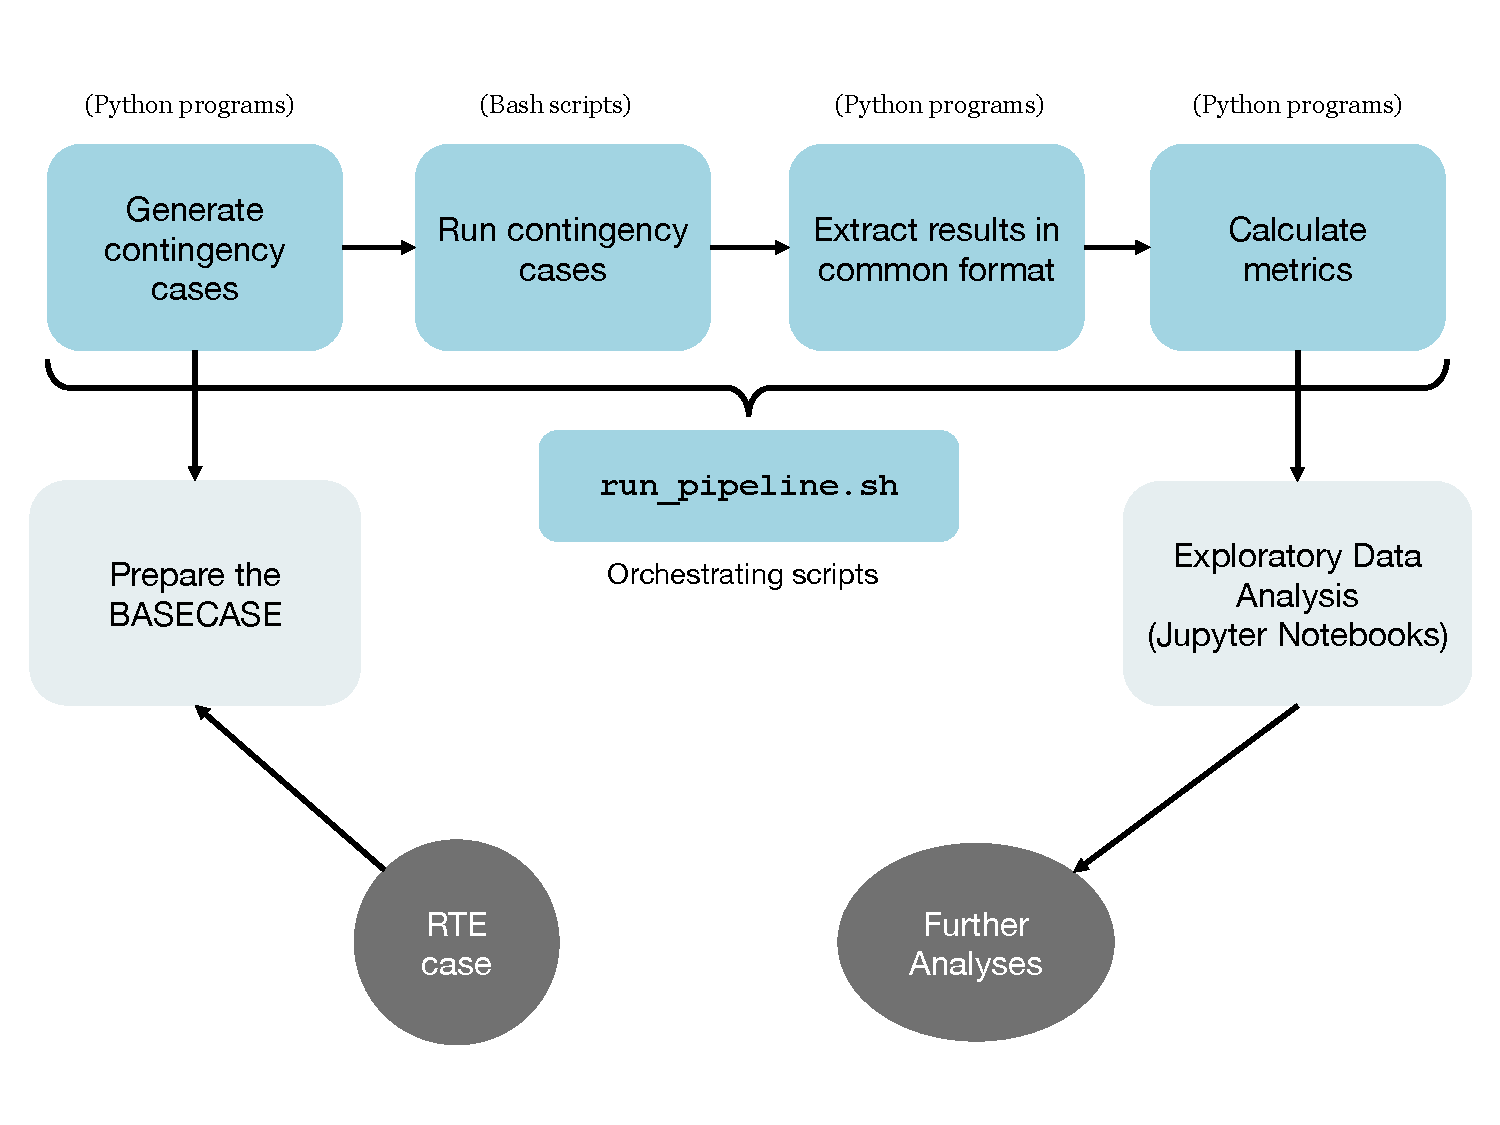
\includegraphics[width=0.48\textwidth]{figs/pipeline}
  \caption{The processing pipeline for validating based on A/B comparison using
    contingency cases.}
  \label{fig:pipeline1}
\end{figure}

For more details than presented here, please consult the source code of the
validation projects under the main repository.\footnote{See:
  \url{https://github.com/dynawo}} The modularity of this design and the use of
scripting languages allows for rapid changes and adaptation to other testing
scenarios. For instance, our implementation creates comparison cases based on
single-element contingencies derived from a common base case, but other users
may want to use a different criterion. This can be achieved by replacing only
the script that generates the set of comparison cases, while the rest of the
pipeline would remain the same.




%%%%%%%%%%%%%%%%%%%%%%%%%%%%%%%%%%%%%%%%%%%%%%%%%%%%%%%%%%%%%%%%%%%%%%%%%%%%%%%%
\section{Metrics and validation}
\label{sec:metrics}

In this context it is assumed that the simulators and their model libraries have
already been validated at the level of simple networks, where device models can
be unitarily tested, isolated from complex collective interactions.  The
challenge is then to perform a quantitative comparison of results on large
scale, real transmission networks. In other words, a verification and validation
of the integrated system is needed.

The difficulties lie on several issues: (a) The sheer number of variables, which
requires one to properly \emph{reduce the data} in order to attempt any
comparison; (b) The fact that the network dynamics is often \emph{sensitive} to
small changes, so that slight differences produced at one point may quickly
amplify down the time line. This is clearly the case in the presence of
thresholding effects, i.e. when a magnitude is close to triggering some actuator
(protection relays, shunts, taps).

The work reported here has shown that it is feasible to devise data-reduction
techniques and metrics to obtain quantitative results, which combined with rapid
exploration and analysis (greatly aided by good visualization choices) allows
one to validate simulators via an extensive set of test cases (in this case,
exhaustive $N$-1 contingency runs).

Conceptually, the following itinerary has been adopted:
\begin{enumerate}
  \item Begin by selecting the \emph{signals} to be
        used for the comparison. Which output variables and events should
        be considered, and which should be discarded? It is indeed
        not manageable nor practical to compare all of them.
  \item Generate a suitable \emph{reduced set of parameters} that characterize
        each type of signal. One is indeed not interested in perfect waveform
        accuracy (in the case of curves), or in perfect event timings (in the case
        of automata events).
  \item Design the \emph{metrics} for measuring the distance between the two
        simulators results in the space of said reduced parameters.
  \item Design effective \emph{visualizations}. This is essential not only
        for the analysis, but as feedback that can guide the design of
        metrics.
  \item Define validation \emph{thresholds} for each class of such
        metrics, which are necessary for establishing hard pass/fail
        criteria (useful when automating tests).
  \item Define one or more \emph{compound scoring} schemes for ranking
        cases. Since the reduced parameters belong to very disparate classes (for
        instance, change in steady-state bus voltages vs.\ changes in Mvar
        peak-to-peak amplitudes), one needs to decide how to combine the metrics
        into a single figure of merit, for the purposes of ranking and sifting
        through the cases to select the ones that need a particular attention.
\end{enumerate}
This process is not linear; it entails feedback loops and repeated cycles until
the research converges on the most adequate or most effective design decisions,
guided by the obtained results.  Each of these steps is discussed in detail in
the following.



\subsection{DynaWaltz metrics}

\subsubsection{Selection of signals}
Here the word \emph{signals} is used to refer to both time-dependent continuous
variables such as voltages and (P,Q) values, as well as discrete events such as
actions fired by control automata. In this paper, signals of the first kind are
called \emph{``curves''}, since this is the terminology used for the output in
both Astre and \Dynawo. For signals of the second kind, they are called
\emph{``automata events''}, or simply automata.

Since DynaWaltz is targeted towards long-term voltage stability studies, our
validation criteria have been focused on the behaviour of the coordinated SVC
systems. This means that, among the huge number of possible signals available
from the simulation, the comparison looks only at these five types:
\begin{itemize}
  \item 4 types of variables related to the SVC systems: pilot bus voltages,
        control K-levels (the SVC gain), and (P,Q) injections of participating
        generators.
  \item the bus voltage(s) of bus(es) involved in the particular
        contingency in each case.
\end{itemize}
Additionally, the criteria also contemplate these types of automata events,
coming from anywhere in the network:
\begin{itemize}
  \item Transformer taps (up/down)
  \item Load-transformer taps (up/down)
  \item Shunt capacitor \& reactor banks (connect/disconnect)
\end{itemize}
The base test cases correspond to the whole of France, down to the \SI{45}{kV}
level.


\subsubsection{Reduced set of parameters}
The aim is to distill a reduced set of parameters that characterize the whole
signal sufficiently well. It is then on these reduced magnitudes that the
metrics are defined.  Since these are transient signals, it would be pointless
to try to match the detailed waveforms; instead, we focused on the most
electrically relevant features.  Eight parameters have been retained, as shown
in Table~\ref{tab:reducedparams}. The last three are meant for automata events
(tap and shunts). Note how they mimic their respective counterparts in
continuous curves: dSS, dPP, and TT,
respectively. Figs.~\ref{fig:tcharacteristics1} and ~\ref{fig:tcharacteristics2}
illustrate all these parameters graphically.

\begin{table}
  \caption{Reduced parameters for time-domain curves and events}
  \centering
  \begin{tabular}{@{}rl@{}}
    \toprule
    \textbf{Parameter} & \textbf{description}                                            \\
    \midrule
    dSS                & ``delta-SS'', difference between initial and final steady state \\
    dPP                & ``delta-PP'', peak-to-peak amplitude during the transient       \\
    TT                 & transient time, the duration of the transient                   \\
    period             & period of the main Prony component of the transient             \\
    damping            & damping of the main Prony component of the transient            \\
    netchange          & net change in tap$^a$ between initial and final steady state    \\
    p2pchange          & peak-to-peak change in tap value during the transient           \\
    numchange          & total number of tap changes$^a$ in the transient                \\
    \bottomrule
    \multicolumn{2}{l}{$^a$ Or in shunt connection status.}
  \end{tabular}
  \label{tab:reducedparams}
\end{table}

\begin{figure}
  \centering
  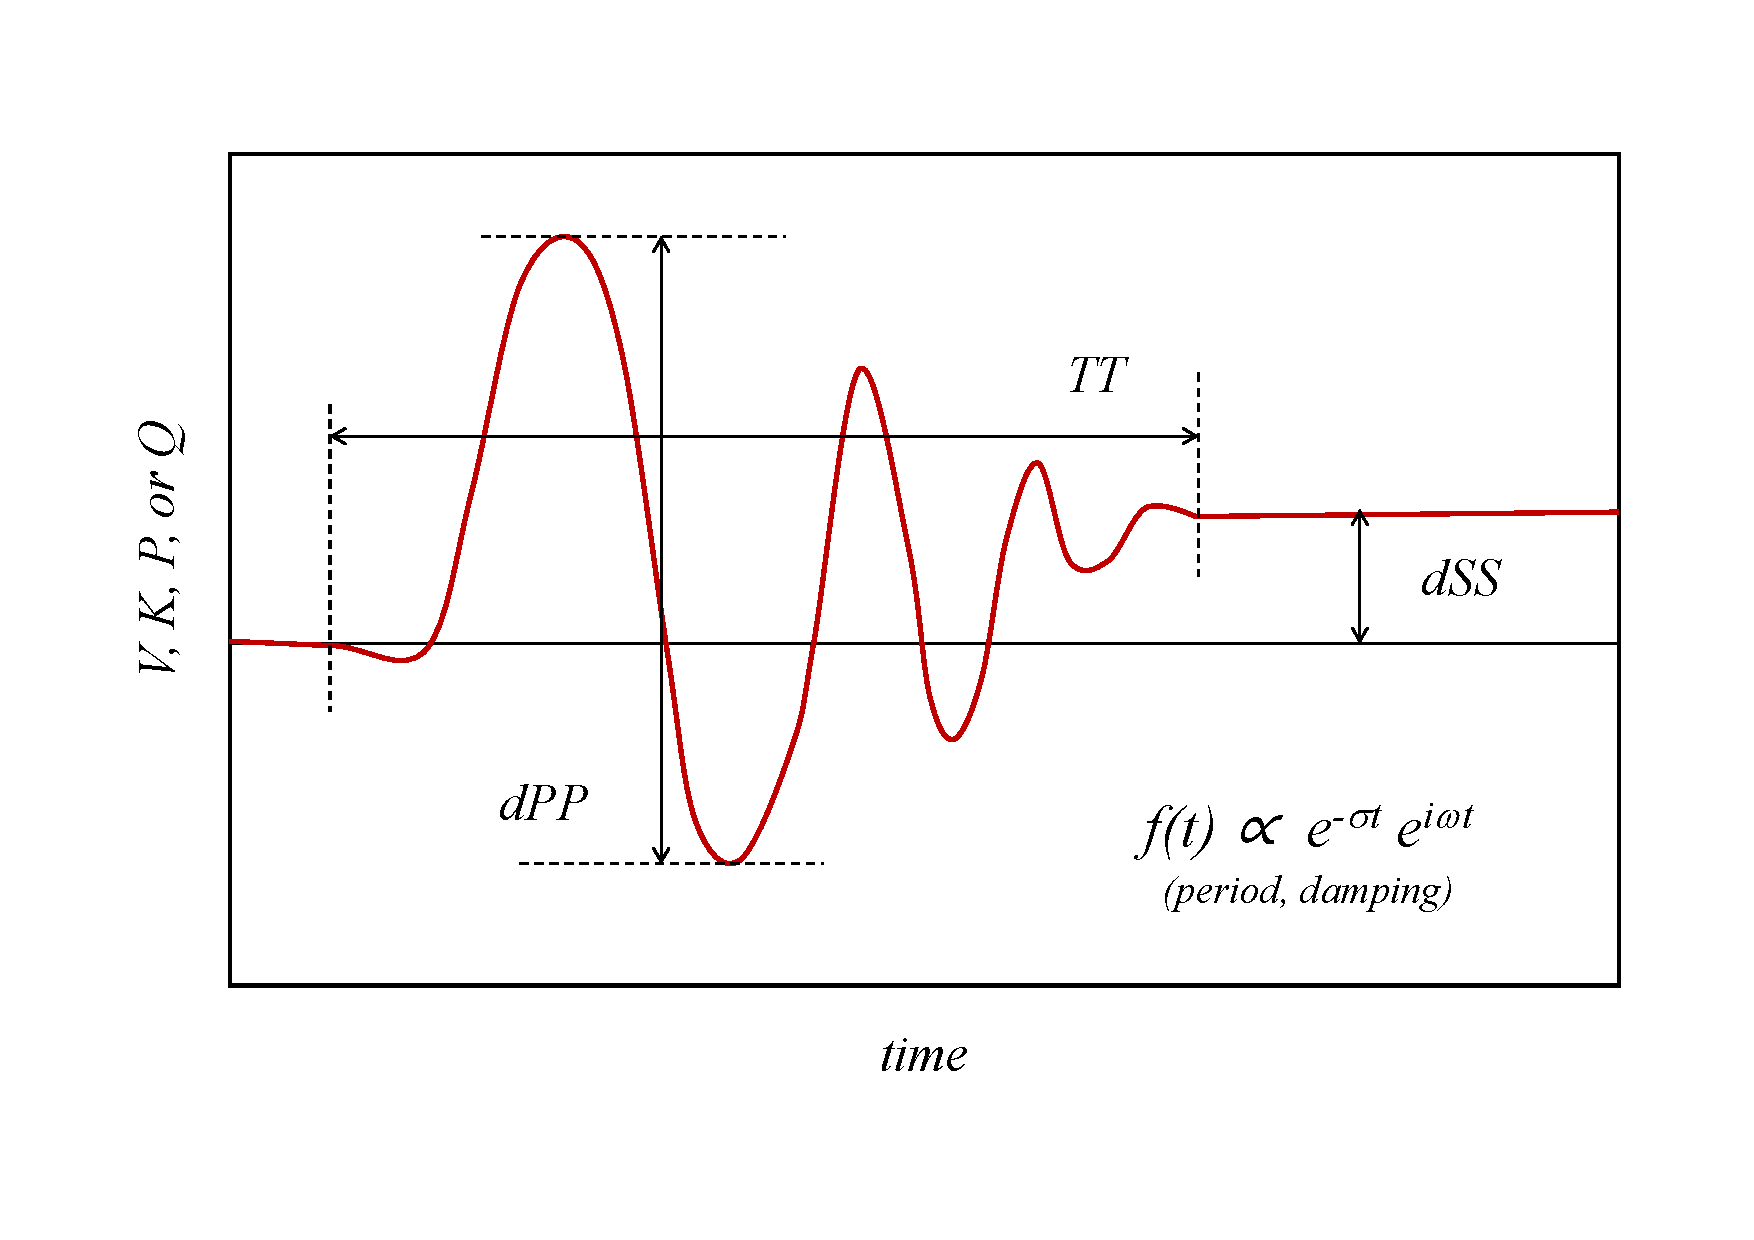
\includegraphics[width=\columnwidth]{figs/transient_characteristics_1}
  \caption{Selection of reduced parameters for characterizing a continuous
    time-dependent transient signal, for the purposes of estimating
    differences.}
  \label{fig:tcharacteristics1}
\end{figure}

\begin{figure}
  \centering
  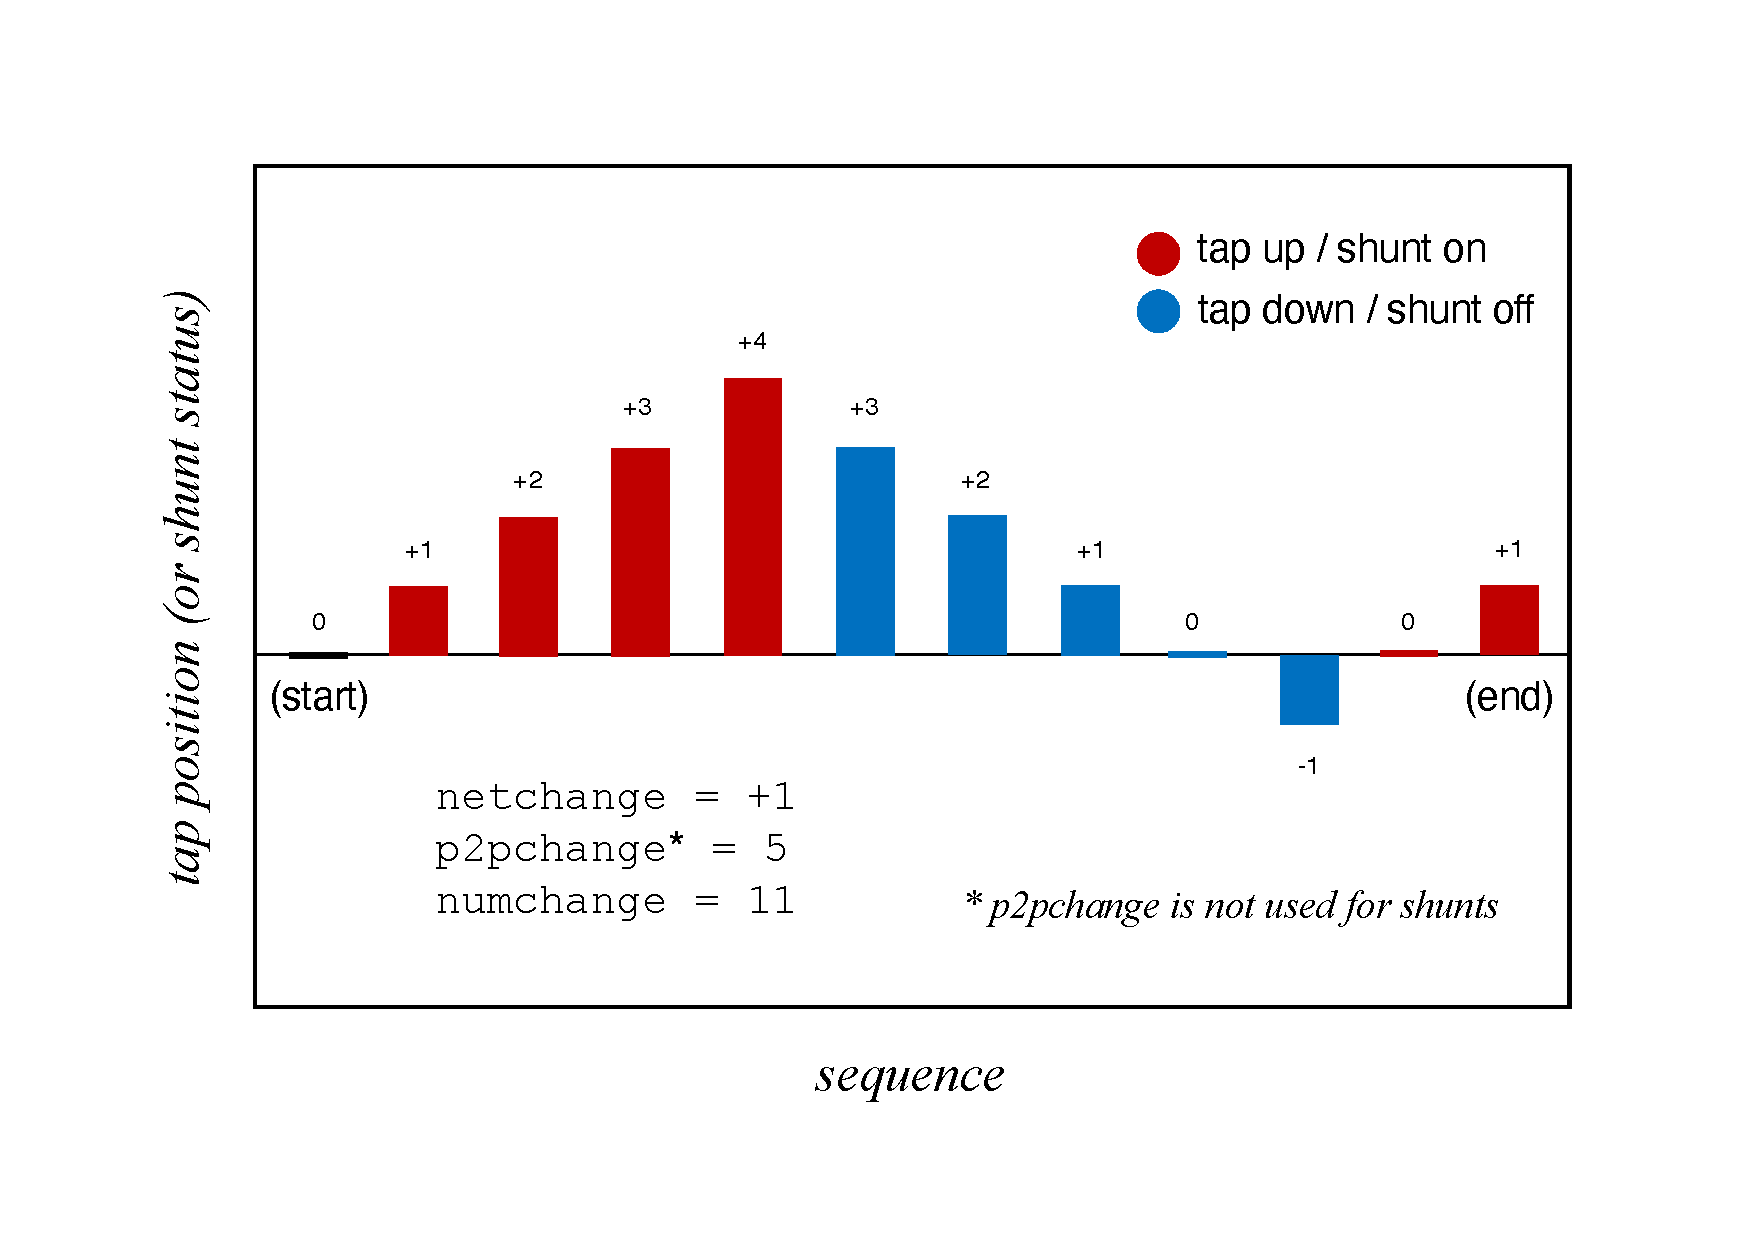
\includegraphics[width=\columnwidth]{figs/transient_characteristics_2}
  \caption{Selection of reduced parameters for characterizing a sequence of
    binary (up/down, on/off) events.}
  \label{fig:tcharacteristics2}
\end{figure}


\subsubsection{Designing the metrics}
\label{sssec:metrics}
For continuous signals, and given the above selected variables and reduced
parameters, there are then 25 different categories (5 variable types x 5
parameters). Within each category, there's usually more than one data point. For
instance, if there are 30 SVC controls in the case file, there will be 30 pilot
bus-voltage dPP values. A metric has to be chosen in order to reduce the
distances to a single number in each variable category. \code{max(abs(diffs))},
which is the max-norm (also called the $L_\infty$-norm) has been chosen.  A
different choice could be \code{mean(abs(diffs))}, which is the $L_1$-norm
divided by the number of variables, but this choice smooths out important
differences when they are local---which is normally the case when running a very
large network.

For automata events, there are 8 categories (3 variable types x 3 reduced
parameters, minus one because p2pchange does not make sense for shunt
events). For these the $L_1$-norm has been chosen, normalized by the total
number of devices (variable tap transformers or switchable shunts). Note that
this is \emph{not} \code{mean(abs(diffs))}, as the denominator is the number of
\emph{all} devices that could potentially produce events, not just the ones that
have actually produced events. This way the metric can tell apart cases where
the number of devices that produced events is very different.


\subsubsection{Compound scoring and validation thresholds}

Compounding the 25+8 different categories into an aggregate metric needs to be
done carefully, in order to deal with the ``apples vs.\ oranges'' problem. Using
relative error for each category sidesteps this problem, but brings others.
From the point of view of validation, it is more natural to define a set of
thresholds, one in each of those categories, using absolute error. One may later
decide whether to assign a global pass/not-pass based on some supra-metric on
the individual pass/not-pass values.


As for the choice of the actual thresholds, one needs to experiment and use
expert judgement. The following thresholds (for absolute errors) have been
retained: \SI{0.01}{pu} for voltages, \SI{5}{MW}/\SI{10}{Mvar} for generators'
(P,Q), and 0.1 (dimensionless) for the SVC gain levels (K). These thresholds
have been applied to characteristics dSS and dPP, which in our experiments have
shown to be the most reliable for these purposes (TT did not seem to have good
sensibility for detecting interesting differences, and the Prony parameters
often showed unreliable values).  Using these, DynaWaltz is found to pass for
more than \SI{80}{\%} of the cases, out of around 20,000 contingency cases using
different base cases.  Note that, except for cases in which bugs were caught, it
is not possible to say that the ``failed'' cases were wrong.  At one point it
becomes impossible to say whether any one simulator solution is the right one
and a more in-depth analysis of both results is necessary.



\subsection{DynaFlow metrics}

Compared to time-domain simulations, the problem of establishing metrics for
comparing power flow solutions is, at first sight, comparatively easier. If one
only focuses on the electrical steady state, the comparison can take place on
the main variables: voltage magnitude at buses, reactive \& active power flows
through branches, and reactive \& active power injections at buses (aggregate
values, to sidestep modelling differences due to merged loads, for instance). We
then use the $L_1$-norm on the differences, either in absolute value or as a
relative error--looking at both is often necessary to uncover the most relevant
differences. As before, this is done separately for each magnitude type and then
compound scoring are defined in order to mix all types into a single figure, so
that a single ranking of the ``top X worst cases'' may be obtained.

More interesting for DynaFlow, though, is to detect discrete events and
activations of automatic controls in the simulation (relays, taps, shunts,
etc.).  When these take place, the differences between Hades and DynaFlow
solutions may be too large and uninformative, since the case conditions may have
diverged too much.  Looking at the timeline of events is then needed in order to
make sense of the results.  Metrics on the differences between power flow
solutions are not helpful in this case---it is simply better to detect the
presence and number of such events.  In particular, it is useful to try
detecting ``root cause'' events, that is, any significant event that in turn
produces several other events in a cascade. This issue is currently being
researched on, since such cause--effect relationships are hard to ascribe from
the raw timeline of events without a proper electrical analysis. A heuristic has
therefore been devised based on the distance between events in time and space
(i.e., distance measured by minimal impedance paths across the grid), with which
one can group these events.  Even with ``false positives'', this kind of
detection is proving useful when investigating cases with large differences.

On the other hand, if one is comparing DynaFlow vs.\ DynaFlow results then all
time-domain information (events and curves) is kept, because then all metrics
and comparisons discussed above for the case of DynaWaltz can be applied here as
well.




%%%%%%%%%%%%%%%%%%%%%%%%%%%%%%%%%%%%%%%%%%%%%%%%%%%%%%%%%%%%%%%%%%%%%%%%%%%%%%%%
\section{Use cases and some sample results}

The pipeline results are shown in both graphical and tabular form in a Jupyter
notebook designed for interaction.  Upon running this notebook, the eyes are
drawn to the plot in Fig.~\ref{fig:bubbleplot1}.  This is one of the most useful
graphs in the notebook; it is an X-Y scatter plot of the reduced magnitude of
choice (dSS, dPP, TT, period, damping), for the variable type of choice:
contingency bus voltages, pilot bus voltages, generator P/Q, or SVC control gain
K-levels. The point color encodes the signal's transient length, while the size
encodes its peak-to-peak amplitude.  When the simulator results are the same,
all dots accumulate on the diagonal. Any differences are clearly visible as
deviations from the diagonal, and the point positions together with their color
and size quickly inform the user about the severity of each contingency case.

\begin{figure}
  \centering
  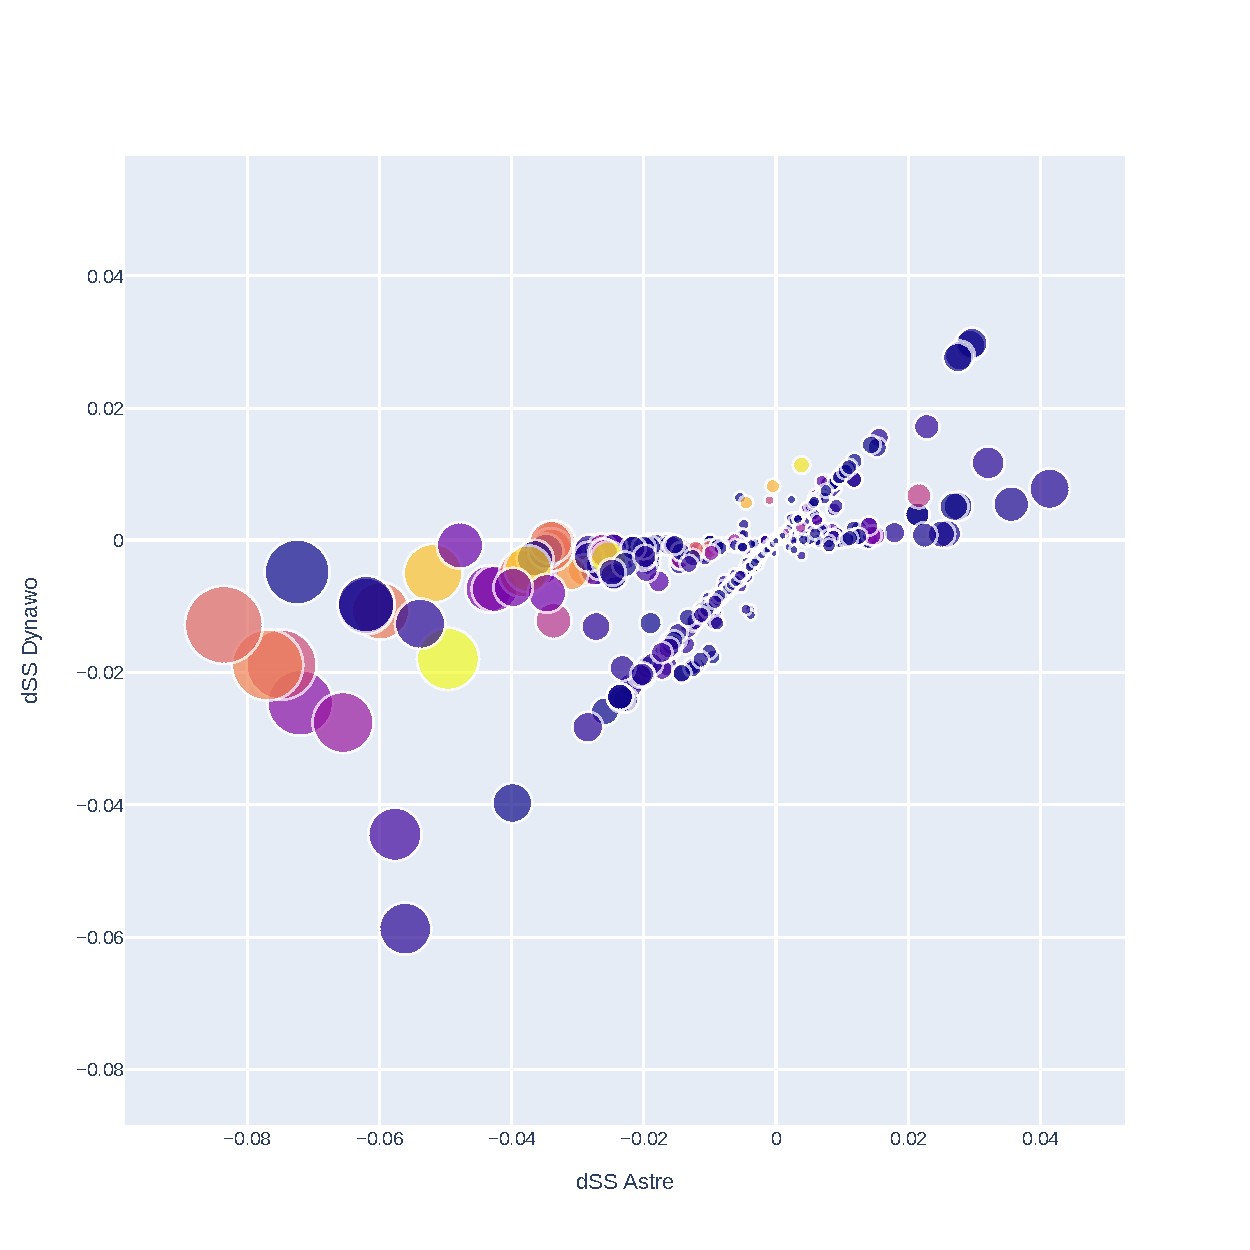
\includegraphics[width=\columnwidth]{figs/Ubus_dSS_GENS_20210211-0930_moreT600}
  \caption{Scatter plot of dSS (change in steady state) of the bus voltage at
    the contingency point, for single-generator contingency cases (exhaustive
    N-1 contingency run: 4,577 cases). The point color encodes the signal's
    transient length; the size encodes its peak-to-peak amplitude.}
  \label{fig:bubbleplot1}
\end{figure}

The power of this plot lies in that it synthesizes the global results.  It is
useful to detect outliers but, more importantly, it is also very effective at
revealing \emph{systematic} differences, that is, patterns in the deviations,
which typically signal some sort of modelling
differences. Fig.~\ref{fig:bubbleplot1} shows an example of this: a significant
number of buses accumulate on a small slope line away from the diagonal,
possibly indicating that the generators near the contingency have some sort of
modelling differences in their voltage control. Hypotheses such as this can
quickly be put to the test by exploring the plot. Hovering over each point
reveals the device's information (ID, voltage level, etc.), and clicking on it
automatically selects the particular contingency case and device signal to plot
on the rest of the graphs. This allows one to quickly drill down to specific
curve graphs and analyze behaviours.

Visual inspection of the curve graphs is always useful as a double-check on a
number of things. For instance, during development many unexpected outliers were
once found, but a quick look at their curves quickly showed that the
steady-state had not yet been achieved at the end of the run. If this happens,
metrics for the differences are bound to be very large and completely
meaningless.  This prompted us to improve the mechanisms for detecting and
flagging unstable cases, so that they can be removed from the comparison.

The tabular information is also there in the notebook, in case one wants to have
access to the actual values and metrics. It is presented in data grid widgets
that allow for sorting and filtering.  These values are also exported to CSV
files, for further analysis in other tools such as Excel.  Data tables are
particularly useful for ranking contingencies by means of the compound scoring
metrics discussed in the previous section.

As a brief example of how to analyze results with the notebook, let us consider
a test run and let us focus on the scatter plot for the dSS values of the
reactive power injection (Q) of all generators participating in the coordinated
SVC systems. Suppose that, unlike Fig.~\ref{fig:bubbleplot1}, there are no
significant patterns of systematic differences, such as lines or clusters off
the diagonal; but there are several outliers sprinkled here and there.  As we
become interested in any of these, we click on one. Then the graphs shown in
Fig.~\ref{fig:curveplot} update to show the specific information for the chosen
generator, in the specific contingency case. The time-domain signal shows indeed
a net difference of about \SI{60}{Mvar} in output, once the new steady state is
reached. The graph stacked on top shows the metrics for the global differences
in discrete events vs.~simulation time (see subsection~\ref{sssec:metrics}
above).  In this case it can be seen that shunt and tap events do not differ
much after the contingency, meaning that the differences in Q developing after
t\,$\sim$\,\SI{1100}{s} must be due to purely local effects. This prompts us to
investigate the model of this generator further, and to try finding whether
there are commonalities shared by other outliers of this kind, etc.

\begin{figure}
  \centering
  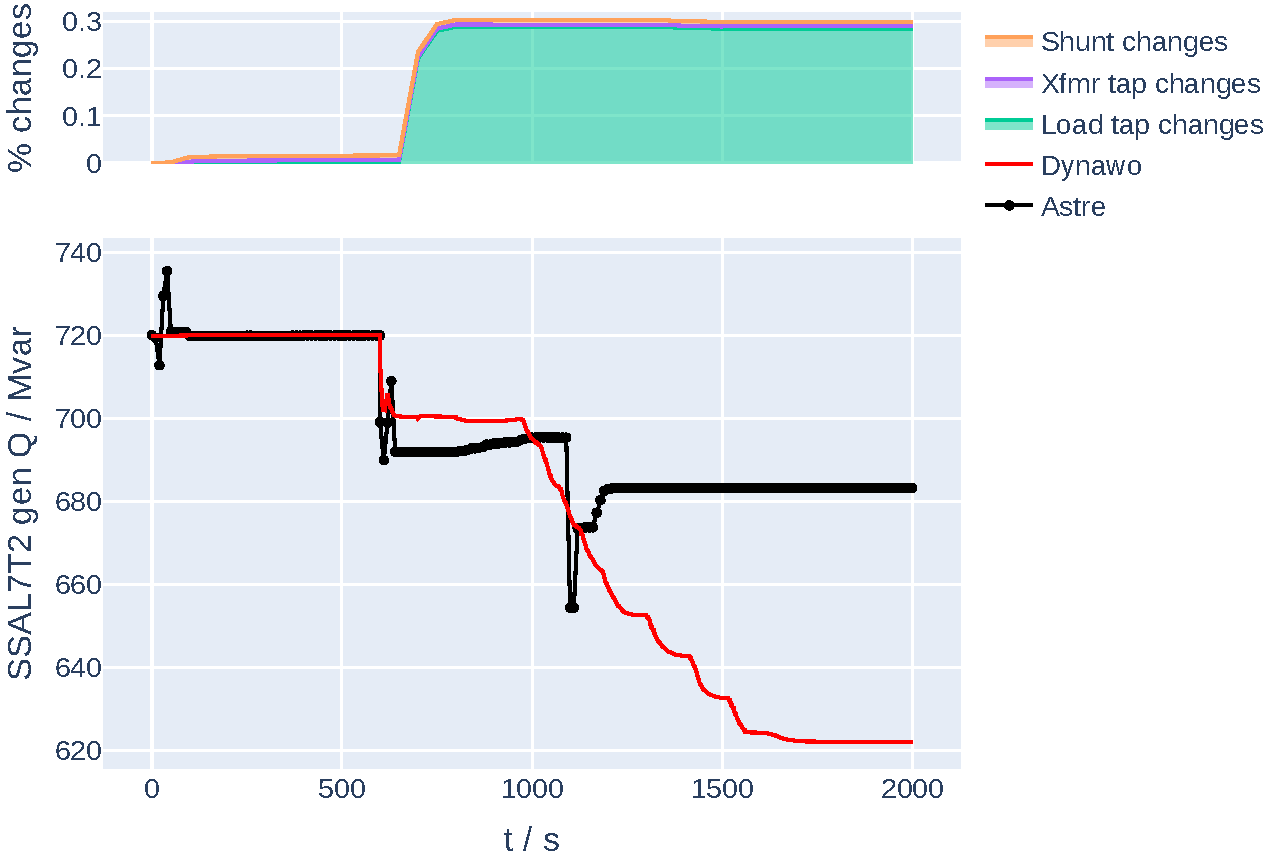
\includegraphics[width=\columnwidth]{figs/Qgen_curve_GENS_20210211-0930_moreT600}
  \caption{Bottom: reactive power of a generator participating in SVC
    (contingency at t\,=\,\SI{600}{s}). Top: metrics for tap and shunt
    events vs.\ time (here ``\%~changes'' is shorthand for ``normalized
    $L_1$-norm based on numchange'').}
  \label{fig:curveplot}
\end{figure}




%%%%%%%%%%%%%%%%%%%%%%%%%%%%%%%%%%%%%%%%%%%%%%%%%%%%%%%%%%%%%%%%%%%%%%%%%%%%%%%%
\section{Conclusion}

A tool has been presented for the testing and validation of time-domain
simulators DynaWaltz and DynaFlow on large, real-world transmission networks.
The proposed approach is based on the extensive simulation of contingency cases,
comparing the results to another already-established simulator. The tool may
also be used for testing new versions of the software (i.e., as a complement to
Unit Testing); or for exploring the effects of different modelling choices,
model parameters, solver parameters, etc.  It can be used for deploying
automated testing procedures to help evolve the software, the models, and their
parameterization.

To meet the challenges involved in measuring the differences between simulations
quantitatively, the relevant outputs were researched, along with the
corresponding metrics. Another challenge was dealing with very large amounts of
data efficiently, and designing effective visualizations for the results. For
this, several modern libraries and rapid development tools from the Python
ecosystem were leveraged.  The tool is expected to be released soon as Open
Source, under the umbrella of all the other \Dynawo{} sub-projects.




%%%%%%%%%%%%%%%%%%%%%%%%%%%%%%%%%%%%%%%%%%%%%%%%%%%%%%%%%%%%%%%%%%%%%%%%%%%%%%%%
\bibliographystyle{IEEEtran}
\bibliography{IEEEabrv,dynawo_validation}




\end{document}

